\documentclass[journal]{IEEEtran}
% EMBER manuscript. Every number traces to paper/results (see NUMBERS_TRACE.md).
\usepackage[T1]{fontenc}
\usepackage{amsmath,amssymb,amsthm}
\usepackage{graphicx}
\usepackage{booktabs}
\usepackage{multirow}
\usepackage{array}
\usepackage{xcolor}
\usepackage{algorithm}
\usepackage{algpseudocode}
\usepackage{tikz}
\usetikzlibrary{arrows.meta,positioning,fit,calc}
\usepackage[hidelinks]{hyperref}
\usepackage{cite}
\usepackage{url}
\usepackage{siunitx}
\sisetup{group-separator={,},group-minimum-digits=4}

\newtheorem{theorem}{Theorem}
\newtheorem{definition}{Definition}
\theoremstyle{remark}
\newtheorem*{remark}{Remark}

\newcommand{\ember}{\textsc{Ember}}
\newcommand{\us}{\,\textmu s}
\newcommand{\Th}{\mathsf{Th}}
\newcommand{\Sig}{\mathsf{Sig}}
\newcommand{\Adv}{\mathrm{Adv}}
\newcommand{\vmax}{V_{\max}}
\newcommand{\B}[1]{B#1}

\hyphenation{Merkle Open-SSL Cloud-Front}

\begin{document}

\title{Post-Quantum Access Tokens for CDNs:\\ Stapling Fixes the Edge, Batching Fixes the Issuer}

% ---- AUTHOR BLOCK (EDITABLE PLACEHOLDER) ----
\author{Dhavan~Arjampudi%
\thanks{D. Arjampudi is with Andhra University, Visakhapatnam, India (e-mail: \emph{[editable]}).}%
\thanks{[Editable: funding statement, ORCID, corresponding-author note.]}}
% ---- END AUTHOR BLOCK ----

\markboth{Manuscript submitted for review (revision 1)}{Arjampudi: Post-Quantum Access Tokens for CDNs}

\maketitle

\begin{abstract}
CDNs gate protected objects with signed URLs and cookies, using either an HMAC key shared with every edge or RSA, ECDSA or Ed25519, which a quantum computer would break. Replacing them with per-token ML-DSA or SLH-DSA signatures yields tokens of \num{3350} to \num{22907} bytes that exceed URL budgets and inflate every segment request. We present EMBER, a CDN profile of Merkle batch signatures: the issuer places all tokens of an epoch in a salted, domain-separated Merkle tree, signs only the root, and each token carries an authentication path. We contribute a threat model stating that HMAC is already post-quantum and that the gain is removing minting secrets from edges; root-dissemination modes for an edge fleet, including root stapling; a security reduction sketch; a measurement study against 13 baselines, among them multi-MAC, delegated Ed25519, KEM-wrapped MAC keys, MTL mode and cached ML-DSA; and a fleet simulator validated against a Go prototype. With $2^{16}$ tokens per epoch an EMBER token is 503~B, against \num{3350}~B for ML-DSA-44. Warm verification takes 2.34\us{} natively, 43$\times$ less than ML-DSA-44 verification but 7.9$\times$ HMAC, and one issuer core produces 1.28 million tokens/s. Over HTTP/2 a session needs 0.144$\times$ the header bytes of split-cookie ML-DSA-44. Stapling lowers the share of simulated requests that wait for a root to 0.049\%. We also report negative results. An adaptive epoch controller performed no better than a fixed 10~ms epoch. Period roll-up removed only 1.4--2.2\% of root misses. A hybrid Ed25519+ML-DSA root raised simulated edge CPU per request by 41.6\%.
\end{abstract}

\begin{IEEEkeywords}
Access tokens, content delivery networks, Merkle trees, ML-DSA, post-quantum cryptography, signed URLs, SLH-DSA.
\end{IEEEkeywords}

\section{Introduction}
\label{sec:intro}

\IEEEPARstart{C}{ontent} delivery networks (CDNs) protect paywalled video, software downloads and other private objects with \emph{access tokens}. An issuer, usually the content owner's login service, gives an authorized client a short-lived token. The token binds a URL prefix, an expiry time and optional client attributes. The client attaches it to every request: as a query parameter (a \emph{signed URL}), as a cookie, or in a header. Any edge server can check the token before serving from cache, without contacting the origin. How many requests one token carries varies widely. A token scoped to a streaming session covers one manifest request and then hundreds of segment requests. A signed URL for a single object may be used only once or twice.

Deployed schemes use one of two approaches. Symmetric schemes such as Akamai's EdgeAuth~\cite{akamai-edgeauth} append an HMAC~\cite{rfc2104} under a key held by every edge. Public-key schemes sign the token: CloudFront key groups accept RSA-2048 or ECDSA P-256 keys~\cite{cloudfront-signers}, and Google Media CDN uses Ed25519~\cite{mediacdn-sig}. HMAC-SHA256 is not threatened by quantum computers, but every verifier can also mint tokens. CDNs already hold many customers' secrets~\cite{liang2014httpscdn,cangialosi2016keysharing}, so a single compromised edge exposes every path the key covers. The public-key schemes keep edges secret-free, but Shor's algorithm~\cite{shor1997} would recover their signing keys from long-lived public keys. Authentication has no harvest-now-decrypt-later exposure. The reason to migrate now is lead time: token formats, SDKs and edge verifiers must change before a cryptographically relevant quantum computer (CRQC) exists, and industry roadmaps target post-quantum authentication by about 2029~\cite{cf2026roadmap}.

The obvious replacement is one FIPS~204 ML-DSA signature per token~\cite{fips204,rfc9964}. It produces a \num{3350}-B token, which every request then repeats. Two remedies are available. \emph{Stapling} detaches the signature and sends it once per connection (M2). \emph{Merkle batch signing}~\cite{merkle1989,batchsig2024,fregly2023mtl} signs one root for many tokens, which our earlier version of this work applied to CDN tokens as EMBER. Review of that version showed that at the operating point we had recommended (per-tenant trees, 10~ms epochs) most trees hold a single token and most of the edge benefit came from detaching the signature. A replay of Meta's public CDN traces~\cite{berg2020cachelib,cachelib-traces} then showed that even this edge verdict holds only when tokens carry many requests. This paper separates the two mechanisms, measures each against strong alternatives, and identifies what decides between them at the edge: the number of requests $K$ a token carries at one verifier.

\emph{Contributions.}
\begin{enumerate}
\item \textbf{A trust and threat comparison} of 13 baselines and M2 (Section~\ref{sec:threat}, Table~\ref{tab:trust}). It covers who can mint tokens after an edge compromise, the post-quantum assumption and token size; HMAC is already post-quantum secure.
\item \textbf{Pooled batching relieves the issuer} (Sections~\ref{sec:res-oprg} and~\ref{sec:res-trace}). EMBER, a CDN profile of MTL-mode and batch signatures rather than a new primitive, pays off when one tree is pooled per issuer key, which the pooled tenants must share, and the pool exceeds about $10^3$ tokens/s at $\Delta=10$~ms. It cuts issuer CPU 19--144$\times$ in simulation. At the full rates implied by the trace, per-content-type trees hold a median of 547 tokens and the issuer needs 0.38--1.08 cores against 177 for per-token signing; the single-token trees we reported earlier appear only at low rates.
\item \textbf{Requests per token decide the edge} (Sections~\ref{sec:res-edge} and~\ref{sec:res-trace}). With session tokens ($K\approx150$), M2 matches HMAC in whole-request edge CPU in a Go prototype and is the smallest post-quantum option on the wire. With one token per object per hour ($K=1.7$--2.4 on the trace), M2 verifies a signature about every second request and pooled EMBER is 28$\times$ cheaper in edge crypto and 4.4$\times$ smaller on the wire. From measured costs we derive the crossover: $K^*\approx48$--154 for CPU and 9--27 for bytes.
\item \textbf{HPACK behavior of real clients} (Section~\ref{sec:res-wire}). Chrome~153 adopts an edge-advertised 64~KiB HPACK table, so a 3.3~KB ML-DSA cookie costs 25.7~B per request; curl/nghttp2 and Go clamp it to 4096~B, yet Go kept the cookie indexed (228~B per request) while curl re-sent it.
\item \textbf{A prototype and a simulator.} The simulator matches the prototype on miss and byte counts in all 12 configurations, and we report where it fails (Section~\ref{sec:res-validate}). The prototype runs M2 with its retry path and pooled EMBER for edge CPU, latency under load, and recovery after cache loss, restarts and undersized caches (Sections~\ref{sec:design} and~\ref{sec:res-edge}).
\item \textbf{Deployment guidance} keyed to $K$, the per-key token rate and who holds the issuer key (Section~\ref{sec:discussion}), including when delegated Ed25519 keys suffice: only if a key cannot be broken within its exposure window, for which published estimates range from 38~h to 10~min per key.
\end{enumerate}

\section{Background and Related Work}
\label{sec:background}

\subsection{CDN Access Tokens}
A CDN token consists of \emph{claims} and an \emph{authenticator}. Typical claims are a URL prefix, an expiry time and optionally a client IP range. Media CDN serializes claims as colon- or ampersand-separated fields followed by \texttt{Signature=}, an unpadded base64url Ed25519 signature~\cite{mediacdn-sig}. EdgeAuth uses \texttt{exp=...\textasciitilde acl=...\textasciitilde hmac=...}~\cite{akamai-edgeauth}. Tokens travel in three places. In a query string, an 8000-octet minimum is recommended for URL support~\cite{rfc9110}, and 2~KB is common legacy practice. In a cookie, RFC~6265 requires at least 4096~B per cookie~\cite{rfc6265}. In a header, servers commonly cap total header size, a configuration assumption we state where we use it. In HTTP/2, HPACK~\cite{rfc7541} can index a repeated cookie, but only if the cookie fits in the dynamic table next to the other changing headers. Section~\ref{sec:res-size} shows that this decides whether large tokens are affordable.

Macaroons~\cite{macaroons2014} add attenuation to HMAC bearer tokens but keep HMAC's shared-secret trust. DPoP~\cite{rfc9449} binds tokens to a client key and is orthogonal to how the token itself is authenticated. Post-quantum Privacy Pass~\cite{policharla2023pqpp} provides unlinkable tokens, but at 85--175~KB per token, for a different goal (anonymity).

\subsection{Post-Quantum Signatures}
FIPS~204 standardizes ML-DSA, with signatures of 2420, 3309 and 4627~B for ML-DSA-44/65/87, and FIPS~205 standardizes SLH-DSA, whose 128s and 128f parameter sets have 7856-B and \num{17088}-B signatures~\cite{fips204,fips205}. RFC~9964 registers ML-DSA for JOSE and COSE~\cite{rfc9964}. Measurements of post-quantum TLS~\cite{sikeridis2020ndss,paquin2020benchmarking,sosnowski2023conext,kampanakis2024ttlb} show that signature \emph{size}, more than CPU, drives the cost of post-quantum authentication. CDNs already deploy ML-KEM key exchange at the edge and toward origins~\cite{akamai2026e2epqc,cf2026pqauthorigins}. KEMTLS replaces handshake signatures with KEMs~\cite{schwabe2020kemtls,celi2021measuring}, but tokens are verified offline and have no handshake to which that idea could apply. Hybrid signatures combine a classical and a post-quantum scheme. We use the AND-combiner, in which both signatures must verify, analyzed by Bindel et al.~\cite{bindel2017hybrid}.

\subsection{Merkle Batch Signing}
Merkle's tree authentication~\cite{merkle1989} underlies every scheme in this subsection. Aguilar-Melchor et al.~\cite{batchsig2024} formalize batch signatures, in which one inner signature covers a Merkle tree of messages, and prove unforgeability and privacy. In their model each batch signature carries the root signature and is evaluated for TLS. TLS batch signing~\cite{draft-batch-signing} follows the same pattern. MTL mode~\cite{fregly2023mtl,draft-mtl-mode} signs \emph{ladders} over a growing message series and authenticates messages by a \emph{condensed} signature, a path to a ladder rung. It targets settings, such as DNSSEC~\cite{draft-slhdsa-mtl-dnssec}, in which verifiers check a subset of a large, evolving series. Merkle Tree Certificates (MTC)~\cite{draft-mtc,cf2025mtc} batch certificate issuance under signed tree heads that relying parties obtain ahead of time. MTAC~\cite{draft-mtac} profiles the same structure for AI-agent identity, and its authors state that it specifies no runtime authorization. Certificate Transparency~\cite{rfc9162} defines the tree shape that MTC and our implementation follow. SPHINCS$^+$/SLH-DSA introduced the tweakable-hash framework with address-based domain separation~\cite{sphincsplus2019} that our node hashing reuses.

\begin{table}[t]
\centering
\caption{Merkle batching approaches compared with EMBER.}
\label{tab:related}
\footnotesize
\setlength{\tabcolsep}{3pt}
\begin{tabular}{@{}p{1.45cm}p{1.95cm}p{1.95cm}p{2.1cm}@{}}
\toprule
 & Root signature per message & Verifiers & Size constraint \\
\midrule
Batch sig.~\cite{batchsig2024} & carried in full & one TLS client & none \\
MTL mode~\cite{draft-mtl-mode} & ladder fetched separately & DNS resolvers & DNS message \\
MTC~\cite{draft-mtc} & tree head distributed ahead & browsers & TLS flight \\
\textbf{EMBER} & disseminated by the CDN: pull, push, roll-up, \textbf{stapled} & thousands of edges, $\sim$150 requests per token & URL (2~KB practice), cookie (4096~B) \\
\bottomrule
\end{tabular}
\end{table}

\subsection{What is New Here}
Searches of the literature and of IETF drafts up to November~2026 found no published scheme that applies Merkle batching to CDN signed URLs or cookies. Table~\ref{tab:related} lists the differences in the setting. Our contribution is therefore not the primitive. It is (i) a token profile that meets URL and cookie budgets, with epoch-bounded validity and revocation, (ii) dissemination of signed roots through the CDN itself, including stapling, and (iii) a measurement study that compares the result with strong symmetric, delegated and cached alternatives. Broader surveys of post-quantum migration~\cite{kampanakis2023vision,alnahawi2024survey} list such application-layer artifacts as open problems.

\section{System and Threat Model}
\label{sec:threat}

\subsection{Entities}
\emph{Issuer $I$.} The tenant's authentication service, or an issuer operated by the CDN, holds the signing key $sk$. $sk$ is an ML-DSA-44/65, SLH-DSA-128s/f or hybrid Ed25519\,+\,ML-DSA-44 key, identified by a key id $\mathit{kid}$. \emph{Root service.} An origin object path from which signed epoch roots and period bundles are served. It is itself cacheable through the CDN's shield tier. \emph{Edges} $E_1,\dots,E_E$ hold $pk$, a root cache and a revocation set. \emph{Clients} authenticate to $I$ (for example at a paywall), obtain a token and then issue a manifest request and $K$ segment requests, normally sticky to one edge.

\subsection{Why Not Simply HMAC?}
HMAC-SHA256 tokens are secure against quantum adversaries. Their weakness is that every verifier can also mint. (i) A single edge compromise (a memory disclosure, an insider, a misconfiguration, partner hardware) yields a key that mints tokens for every edge and every path the key covers. (ii) A content owner using several CDNs must share the minting secret with each vendor, and each vendor can mint tokens that the others accept. (iii) There is no issuer accountability. Public-key tokens give edges only $pk$. We do not overstate the benefit. A compromised edge can already serve anything it caches without checking tokens, so asymmetric tokens remove only \emph{lateral} minting: tokens accepted by other edges, other CDNs or other tenants. Table~\ref{tab:trust} in Section~\ref{sec:results} quantifies this blast radius for every baseline.

\subsection{Adversary}
The adversary $\mathcal{A}$ (i) controls the network between clients and edges and can replay observed tokens; (ii) may compromise \emph{any subset} of edges and shields, learning their full state and injecting roots into their caches; (iii) is a legitimate client of any tenant and obtains arbitrarily many tokens for claims of its choice, while leaf salts remain issuer-chosen; and (iv) is quantum. It can run Shor's algorithm against any public key and generic quantum search against the hash function. $\mathcal{A}$ does not obtain the issuer's $sk$. Issuer compromise is handled by key rotation via $\mathit{kid}$. Theft and replay of bearer tokens are unchanged from the status quo and are mitigated by the same means: IP or ASN claims, short validity, and optionally a DPoP-style key-hash claim~\cite{rfc9449}.

\subsection{Goals and Requirements}
\textbf{G1 (unforgeability):} no efficient (quantum) $\mathcal{A}$ makes an honest edge accept claims that $I$ never issued or has revoked, even if all other edges are compromised. \textbf{G2 (edge non-minting):} edges hold no secret. \textbf{G3 (bounded validity):} an edge rejects a token whose expiry exceeds $T_{\text{start}}(e)+\Delta_e+\vmax$ (plus a clock-skew tolerance $\tau$). \textbf{G4 (sibling privacy):} an authentication path reveals nothing about other clients' claims. \textbf{G5 (availability):} an edge that cannot obtain a root fails closed.

Operational requirements are: \textbf{R1}, tokens fit URL and cookie budgets with margin; \textbf{R2}, per-request edge cost close to HMAC; \textbf{R3}, no minting secret at edges; \textbf{R4}, bounded issuance latency; \textbf{R5}, revocation; \textbf{R6}, negligible dissemination bandwidth and rare root-miss waits; and \textbf{R7}, a clear security reduction.

\section{Design Space}
\label{sec:design}

All schemes authenticate the same canonical claim string, so only the authenticator and its delivery differ. Fig.~\ref{fig:arch} shows the two post-quantum designs this paper focuses on.

\begin{figure}[t]
\centering
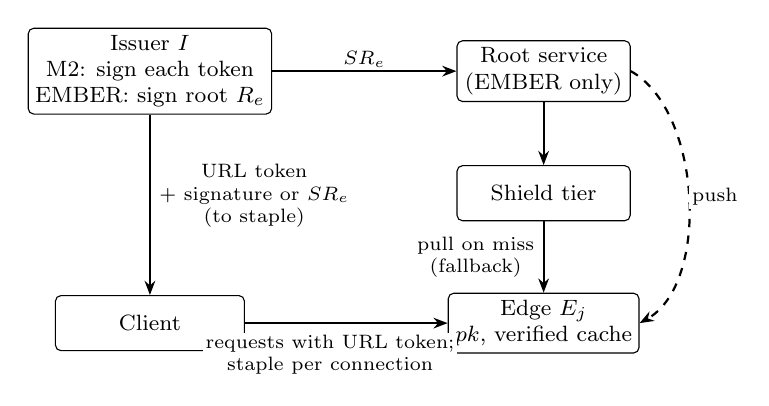
\begin{tikzpicture}[
  font=\footnotesize,
  box/.style={draw, rounded corners=2pt, align=center, minimum height=0.7cm, inner sep=2.5pt, fill=white},
  lab/.style={font=\scriptsize, align=center, fill=white, inner sep=1pt},
  arr/.style={-{Stealth[length=1.8mm]}, thick},
  darr/.style={-{Stealth[length=1.8mm]}, thick, dashed}]
\node[box, minimum width=2.4cm] (iss) at (0,0) {Issuer $I$\\ M2: sign each token\\ EMBER: sign root $R_e$};
\node[box, minimum width=2.2cm] (rs) at (5.0,0) {Root service\\ (EMBER only)};
\node[box, minimum width=2.2cm] (sh) at (5.0,-1.55) {Shield tier};
\node[box, minimum width=2.2cm] (edge) at (5.0,-3.2) {Edge $E_j$\\ $pk$, verified cache};
\node[box, minimum width=2.4cm] (cli) at (0,-3.2) {Client};
\draw[arr] (iss) -- node[lab, above]{$SR_e$} (rs);
\draw[arr] (rs) -- (sh);
\draw[arr] (sh) -- node[lab, left=2pt]{pull on miss\\(fallback)} (edge);
\draw[darr] (rs.east) .. controls +(0.9,-0.5) and +(0.9,0.5) .. node[lab, right]{push} (edge.east);
\draw[arr] (iss) -- node[lab, right=2pt, pos=0.45]{URL token\\$+$ signature or $SR_e$\\(to staple)} (cli);
\draw[arr] (cli) -- node[lab, below=3pt, pos=0.42]{requests with URL token;\\ staple per connection} (edge);
\end{tikzpicture}
\caption{Stapled post-quantum tokens. In M2 the client staples its token's ML-DSA signature on the first request of each connection. In EMBER it staples the signed epoch root $SR_e$ (MTL's ``full'' signature) and the URL carries a Merkle path. Pull from the root service through the shield tier and push are EMBER fallbacks.}
\label{fig:arch}
\end{figure}

\subsection{Per-Token Signatures, Cached or Stapled}
\textbf{B5/B6} put an ML-DSA-44/65 signature in every token. \textbf{B5v} adds an edge cache of verified tokens, keyed by SHA-256 of the token, so verification runs once per (token, edge). The 3.3~KB token is still sent and hashed on every request. \textbf{M2} (stapled per-token ML-DSA-44) separates the signature from the token. The URL token is the claims followed by \texttt{:S=}b64url($\mathit{kid}\,\|\,$16-B nonce). On the first request of each connection, the client sends the 2,420-B signature over (claims, nonce) in a header. We use the connection as the staple unit because a client can observe connections but not edges. The edge verifies the signature, caches $H(\mathit{ref}\,\|\,\text{claims})$ as verified until the token's expiry, and from then on hashes about 138~B per request.

\emph{Recovery.} M2 has no pull fallback. An edge that holds no valid entry for a token answers with 401 and a \texttt{Staple-Required} hint, and the client retries the same request with the signature header. This happens after a cache eviction, an edge process restart, or a server that does not share the cache. Our prototype implements the hint as a 403 with \texttt{X-Reject: staple required}. A recovery costs one client--edge round trip (20.98~ms mean in our testbed), a \num{3242}-B HTTP/1.1 header line, and one ML-DSA-44 verification (100.9\us). Because clients staple on every new connection, recovery is needed only when an edge loses an entry for a connection that is still open. The edge state is small. In the prototype an entry is a 16-B key plus an 8-B expiry (24~B, excluding hash-table overhead), and it lives at most until the token expires ($\le\vmax=1$~h). At the busiest simulated edge, new (token, edge) pairs arrive at 165.8/s ($\bar\lambda=2000$/s) and \num{1658}/s (\num{20000}/s). This bounds the live set at 0.60 and 5.97 million entries, or 14.3 and 143~MB of payload. An edge that retains this state never needs recovery for unexpired tokens. We did not measure how often recovery occurs. M2 is the $N=1$ special case of EMBER, and it is also B5v without the per-request resend. Its security is the EUF-CMA security of ML-DSA plus the collision resistance of the cache key.

\subsection{EMBER: Pooled Epoch-Merkle Batching}
\label{sec:ember}
\emph{Notation.} $H$ is SHA-256 truncated to $n\in\{16,32\}$ bytes. The tweakable hash is $\Th(T,x)=\mathrm{trunc}_n(H(T\|x))$ with a fixed-length 26-B tweak $T=\texttt{"EMBERv1\textbackslash0"}\|\mathit{kid}\|e\|\mathit{type}\|\ell\|j\|\mathit{tenant}$, so every node position of every epoch is a distinct function~\cite{sphincsplus2019}. Leaf $i$ of epoch $e$ is $L_i=\Th(T_{\textsc{leaf}}(e,i),\,r_i\|\mathrm{enc}(c_i))$, where $r_i$ is a 128-bit salt that the issuer draws \emph{after} it receives the claims $c_i$. Inner nodes are $\Th(T_{\textsc{node}}(e,\ell,j),\,\text{left}\|\text{right})$, and the tree has the RFC~9162 shape~\cite{rfc9162}, with depth $d=\lceil\log_2N_e\rceil$. The signed epoch root is $SR_e=(\mathit{kid},e,T_{\text{start}},\Delta_e,N_e,R_e,\sigma_e)$, where $\sigma_e=\Sig(sk,\texttt{"EMBER-root"}\|\mathit{kid}\|e\|T_{\text{start}}\|\Delta_e\|N_e\|R_e)$ is ML-DSA-44 with the FIPS~204 context string \texttt{EMBER-root}. In the hybrid variant, $\sigma_e$ is an Ed25519 signature and an ML-DSA-44 signature over the same message, and both must verify.

\emph{Token.} The URL token is \texttt{URLPrefix=\ldots:Expires=\ldots:} \texttt{Tenant=\ldots:E=}\textit{blob}, where the blob is the base64url encoding of version, algorithm, $\mathit{kid}$, $e$, $i$, $r_i$ and the path, $30+nd$ raw bytes in all. With $c_{\text{enc}}$ bytes of encoded claims,
\begin{equation}
S_{\text{tok}}=c_{\text{enc}}+3+\lceil 4(30+nd)/3\rceil .
\label{eq:size}
\end{equation}
Our encoder implements Eq.~\eqref{eq:size}. With a 60-character path ($c_{\text{enc}}=118$) it yields 161, 268, 332 and 460~B for $N=1$, $2^5$, $2^8$ and $2^{14}$, against 148~B for M2.

\emph{Issuance and pooling.} The issuer collects requests for $\Delta$ seconds, or until a count cap $N_{\max}$ is reached, and then closes the epoch. Closing builds the tree ($2N-1$ hashes), signs the root once, and returns to each client its token and $SR_e$. Before the epoch or index counters would wrap, the issuer rotates $\mathit{kid}$. The unit of batching is the \emph{pool}, meaning the set of tenants that share a tree. Batching saves signatures only when a pool receives many tokens per $\Delta$. With $P$ pools the issuer makes at most $P/\Delta$ signatures per second, independent of the token rate. Pooling lets one issuer key mint tokens for every tenant in the pool. It is therefore appropriate only when the tenants already delegate issuance to the CDN or belong to one trust domain. Tenant is part of the claims and of the leaf tweak, so leaves cannot be replayed across tenants.

\emph{Verification} is given in Algorithm~\ref{alg:verify}. Revocation uses short $\vmax$ (1~h by default), signed lists of revoked $(e,i)$ pairs at 8~B each, or withdrawal of a whole epoch root.

\begin{algorithm}[t]
\caption{Edge verification of an EMBER token}
\label{alg:verify}
\small
\begin{algorithmic}[1]
\Procedure{Verify}{$\mathit{tok},\mathit{url},\mathit{now}$}
  \State parse claims $c$ and $(\mathit{kid},e,i,r,\text{path})$; reject if malformed or $\mathit{kid}$ unknown
  \State reject if $\mathit{now}>c.\mathit{Exp}+\tau$ or $c.\mathit{Exp}>T_{\text{start}}(e)+\Delta_e+\vmax+\tau$
  \State reject if URL prefix or IP binding fails, $(e,i)$ revoked, or $i\ge N_e$
  \State $R\gets\mathit{RootCache}[\mathit{kid},e]$
  \If{$R=\bot$}
    \If{a stapled $SR_e$ is present} verify $\sigma_e$ (per-client rate limit); cache
    \Else{} fetch $SR_e$ via shield (coalesced, negative-cached); verify; cache
    \EndIf
    \State on failure or timeout: \Return reject \Comment{fail closed}
  \EndIf
  \State $x\gets\Th(T_{\textsc{leaf}}(e,i),r\|\mathrm{enc}(c))$
  \For{each sibling $s_\ell$ in path} $x\gets\Th(T_{\textsc{node}}(e,\ell,\cdot),\mathrm{order}(x,s_\ell))$
  \EndFor
  \State \Return $x\stackrel{\text{ct}}{=}R$
\EndProcedure
\end{algorithmic}
\end{algorithm}

\subsection{Root Dissemination}
\label{sec:dissem}
An edge cannot verify an EMBER token until it holds $R_e$. There are four ways to get it there. \textbf{Pull}: the edge fetches $SR_e$ through the shield on a miss, with coalesced fetches. \textbf{Push}: the issuer fans each root out to all edges, at fleet bandwidth $BW_{\text{push}}=T_{\text{active}}\,E\,(|\sigma|+40)/\Delta$ for $T_{\text{active}}$ active pools. \textbf{Period roll-up}: every $m$ epochs one signed bundle lists the $m$ roots. \textbf{Stapling}: the client sends $SR_e$ in a header, either only on the session's first request (\emph{staple-first}, our earlier design) or on the first request of every connection (\emph{staple-all}). In our workload a session opens one connection per edge it uses, so staple-all equals stapling on every new edge contact, which is how the simulator models it. The stapled header is the 2,461-B signed root, \num{3298}~B as an HTTP/1.1 header line. With staple-all, verification does not depend on the root service, which matters because edges fail closed. During an outage of the root service or the shield tier, pull-only edges reject every token of an epoch they have not cached, while stapled tokens still verify. M2 and staple-all EMBER instead depend on the edge retaining verified entries, or on the recovery retry. For Poisson token arrivals in pull mode, the expected number of root misses per token at edges with traffic shares $w_v$ is
\begin{equation}
M(\Delta)=\frac{1}{\lambda\Delta}\sum_{v=1}^{E}\bigl(1-e^{-\lambda\Delta w_v}\bigr).
\label{eq:miss}
\end{equation}
The added delay per token is $D=\Delta/2+t_{\text{epoch}}+M(\Delta)F_{\text{miss}}$, where $F_{\text{miss}}$ is the root round trip plus $t_v$ (pull), or $t_v$ alone (stapling). When $\lambda\Delta\ll E$, $M\to1$: almost every token is the first at its edge in its epoch, so only stapling or push avoids the round trip.

\subsection{Security}
\label{sec:security}
\begin{theorem}
\label{thm:uf}
Suppose an adversary $\mathcal{A}$ makes $q_h$ queries to $\Th$ and the issuer evaluates $\Th$ at $p\le\sum_e(2N_e-1)$ tree positions. Then there exist $\mathcal{B}_1,\mathcal{B}_2$ with about the same running time such that
$\Adv^{\mathrm{uf\text{-}tok}}_{\ember}(\mathcal{A})\le\Adv^{\mathrm{euf\text{-}cma}}_{\Sig}(\mathcal{B}_1)+\Adv^{\mathrm{sm\text{-}tcr}}_{\Th,p}(\mathcal{B}_2)$.
\end{theorem}
\begin{IEEEproof}[Proof sketch]
Let $R^*$ be the root the edge used. If the issuer never produced $R^*$ for $(\mathit{kid},e^*)$, then the verified $\sigma$ is a forgery, which $\mathcal{B}_1$ outputs. Otherwise $R^*=R_{e^*}$ is honest, and since $i^*<N_{e^*}$ is enforced, an honest leaf $i^*$ exists whose claims differ from $c^*$. The honest and adversarial hash chains start from different inputs and reach the same root. So at some position they have different inputs and equal outputs under the same tweak. The honest input there contains the salt $r_{i^*}$, which was chosen after $\mathcal{A}$ fixed $c_{i^*}$, or a value derived from it. $\mathcal{A}$ therefore hits a fixed honest target, which is an sm-tcr break; distinct tweaks rule out multi-target speed-ups~\cite{sphincsplus2019}. Replays across epochs, tenants or $\mathit{kid}$ change the tweak and fall into the second case.
\end{IEEEproof}
This is a sketch, not a new proof. For $n=32$, plain collision resistance suffices, matching batch signatures~\cite{batchsig2024}. The root and period-bundle signatures use distinct context strings. The hybrid root is an AND-combiner, at least as strong as its stronger component~\cite{bindel2017hybrid}. sm-tcr is defined for a keyed hash family. Our tweak contains $\mathit{kid}$ and the epoch but no random public seed (SLH-DSA's PK.seed). We therefore recommend adding a 16-B random seed per $\mathit{kid}$ to the tweak, carried in $SR_e$. This adds 16~B to the staple and nothing to tokens. We did not measure this variant. \emph{Truncation:} ML-DSA-44 is a category-2 parameter set~\cite{fips204}. With $n=16$, the generic second-preimage bound is about $2^{128}$ classically and $2^{64}$ with Grover. The \emph{token} therefore offers category-1 security, the same generic level as SLH-DSA-128's 16-B hashes~\cite{fips205}. Use $n=32$ for higher categories (+341~B at $N=2^{16}$). The issuer-chosen salt is mandatory, because $\mathcal{A}$ must not control both inputs of a collision.

\emph{Other threats.} Downgrade: once a tenant has switched, edges must reject classical tokens for that tenant. Privacy: $N_e$ in a public root leaks issuance volume, and the pair $(e,i)$ identifies a token, as a per-token signature already does. Padding the tree to $2^d$ hides the volume. It slowed our Python issuer by 12.45\% at $N=1000$, but the worst case is $N=2^k+1$, where the analytic native cost rises by 38.9\% at $N=2^{14}+1$. DoS: tokens naming fake epochs trigger root fetches, and fake staples trigger signature verifications (Section~\ref{sec:res-other}). Replaying a \emph{valid} staple costs nothing at an edge that has the root cached, and costs at most one verification per $(\mathit{kid},e)$ elsewhere. Per-client limits bound both cases.

\section{Evaluation Methodology}
\label{sec:method}

\begin{table}[t]
\centering
\caption{Schemes compared: 13 baselines, M2 and variants. All are implemented in Python; $\dagger$ marks schemes that are also in the Go prototype.}
\label{tab:baselines}
\footnotesize
\setlength{\tabcolsep}{3pt}
\begin{tabular}{@{}lp{6.6cm}@{}}
\toprule
ID & Scheme \\
\midrule
B1$^\dagger$ & HMAC-SHA256, key shared with all edges (EdgeAuth-like) \\
B2$^\dagger$, B3$^\dagger$, B4 & Ed25519 (Media CDN); ECDSA P-256 and RSA-2048 (CloudFront) \\
B5$^\dagger$, B6$^\dagger$, B7, B8 & per-token ML-DSA-44/65, SLH-DSA-128s/128f \\
B9$^\dagger$ & per-token hybrid Ed25519 + ML-DSA-44 \\
B10 & multi-MAC: one 16-B HMAC tag per verifier domain, $k\in\{1,3,10\}$ \\
B11$^\dagger$ & delegated Ed25519 key, certified per lifetime $L$ by ML-DSA-44 \\
B12$^\dagger$ & per-epoch HMAC key wrapped with ML-KEM-768~\cite{fips203} to each edge \\
B13 & MTL mode, one series per key~\cite{draft-mtl-mode} \\
\textbf{M2}$^\dagger$ & \textbf{stapled per-token ML-DSA-44} (Section~\ref{sec:design}) \\
\midrule
B5v$^\dagger$, B5c & B5 with an edge verify cache; B5 split over two cookies \\
O1$^\dagger$/O2/O3/O4$^\dagger$ & EMBER, $n=16$/$n=32$/SLH-DSA-128s root/hybrid root \\
\bottomrule
\end{tabular}
\end{table}

\textbf{Schemes.} Table~\ref{tab:baselines} lists the 13 baselines (B1--B13), M2 and the variants. Macaroons and DPoP are discussed only qualitatively (Section~\ref{sec:background}). In B13 the MTL series grows over $\vmax$. An MTL series restarted at every epoch is structurally the same as EMBER, so we do not list it separately.

\textbf{Testbed and implementations.} All experiments ran on one KVM guest with 4 vCPUs (Xeon at 2.1~GHz, AVX-512, SHA-NI) and 15~GB of RAM, running Linux~6.18. Primitive costs come from a native C benchmark against OpenSSL~3.5.4 (EVP interface, 5 fresh processes pinned to one core). We report the median of the run medians together with the [min--max] of the run medians. The Go prototype uses Go~1.24.7 and cloudflare/circl~1.6.1, and Python (pqcrypto~1.0.0) is a secondary source. We ran the native suite twice, separated by a VM reboot. Absolute values differ by 15--20\% (ML-DSA-44 verification took 100.9 vs.\ 122.3\us), while ratios are stable. All tables and all simulations use the second run, except the epoch-controller study and the simulator consistency check (Appendix~\ref{app:secondary}). Rerunning the parameter sweep with second-run costs left misses unchanged bit for bit and moved $D$ by at most 0.1~ms, so the controller conclusions, whose effects are all far below 10~ms, cannot change.

\textbf{Prototype.} The Go prototype consists of an edge (\texttt{net/http}; root cache with coalescing and a negative cache; optional verified-token cache; $V$ virtual edges), an issuer and root service, and an open-loop load generator. Client, edge and origin run in separate network namespaces joined by userspace link emulators (\texttt{netem} is unavailable): one-way delays of 10~ms and 37.5~ms, 1~Gbit/s, MTU 1500. \emph{P1} measures edge CPU cost. It is a closed loop over the edge namespace's loopback with the edge on one core, 64 keep-alive connections, $K=150$ requests per token and 5 runs. Its primary metric is edge CPU time per HTTP request. P1 measures CPU, not the network. \emph{P3} measures root dissemination over the emulated links with $V\in\{10,50\}$ virtual edges, $\Delta\in\{0.1,1,10\}$~s and $\lambda\in\{20,200\}$/s, in pull and staple-first modes: 12 configurations, each with a 60~s window and 5 runs. The prototype has no M2 or staple-all dissemination run and no pooled-EMBER run. \emph{P2} measures latency under load (Appendix~\ref{app:secondary}). TLS is not included.

\textbf{Wire bytes and real clients.} Request-header bytes per session (1 manifest and 150 segment requests) are encoded with Go's HPACK at 4096-B and 64~KiB tables. To observe real encoders, a raw-frame HTTP/2 server advertises a table size and logs each request's header-block length while a client fetches 150 objects with a \num{3311}-B cookie value. The clients are headless Chrome~153 (3 runs), curl~8.5.0/nghttp2~1.59.0 and the Go x/net client. We did not test Firefox or Safari.

\textbf{Fleet simulator.} The simulator is an epoch-level Monte Carlo engine driven by the native costs. Its default fleet has $E=500$ edges with Zipf(0.8) traffic shares and 50 shields, and $T=1000$ tenants with Zipf(1.0) rates and aggregate rate $\bar\lambda\in\{200,2000,\num{20000}\}$/s. Sessions have $K$ geometric with mean 150, 4~s apart, and each segment is re-routed to another edge with probability $p_{\text{move}}=0.0005$ (about 7\% of sessions move once). RTTs are lognormal: edge--shield 15~ms, shield--root 60~ms, token receipt to first request 120~ms. All of these are assumptions; the sensitive ones are swept (Appendix~\ref{app:secondary}). The pooling policies are per-tenant trees, 8 shards, 10 or 50 regional pools, and one pool per issuer key. Each is run with a fixed $\Delta$, work-conserving closing (WC, close whenever the signer is idle) or M2. CIs are Student-$t$ 95\% intervals over 5 seeds with common random numbers. Unless stated, their half-widths are below 1\% of the mean.

\textbf{Hypotheses.} We fixed hypotheses H1--H9 in the design document before running any experiment (repository commit \texttt{3148c65}, 2026-11-05 18:07 UTC). Appendix~\ref{app:hyp} reports every outcome.

\section{Results}
\label{sec:results}

\subsection{Token Size and Bytes on the Wire}
\label{sec:res-size}

\begin{figure}[t]
\centering
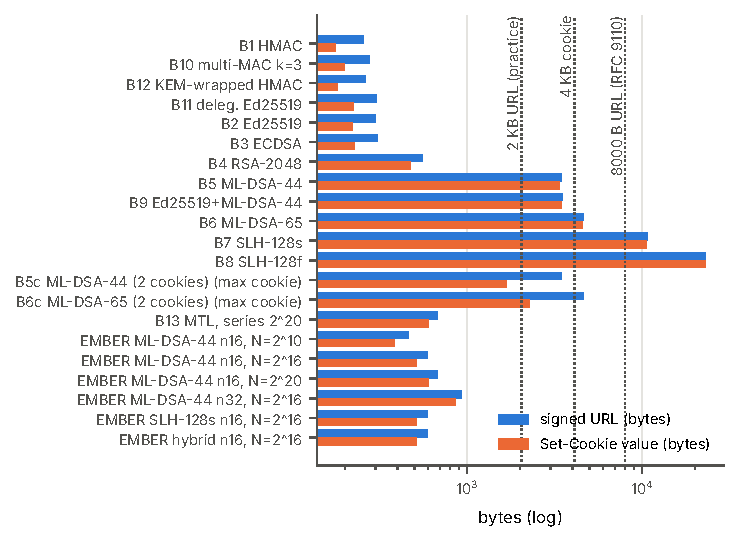
\includegraphics[width=\columnwidth]{figures/fig2_token_sizes.pdf}
\caption{Encoded token size per scheme (measured; 60-character path). Vertical lines: 2~KB URL practice, 4096-B cookie~\cite{rfc6265}, 8000-B URL recommendation~\cite{rfc9110}.}
\label{fig:sizes}
\end{figure}

Fig.~\ref{fig:sizes} shows measured token sizes. Per-token post-quantum signatures do not fit: B5 (ML-DSA-44) is \num{3350}~B, B6 \num{4535}~B, B7 \num{10598}~B and B8 \num{22907}~B, and the B9 hybrid is \num{3435}~B. Under a lognormal URL-path assumption (median 80 characters), no B5 or B6 signed URL fits in 2~KB, no B6 cookie fits in 4096~B, and B7/B8 fit no limit. Classical tokens are 166~B (B1), 209~B (B2) and 465~B (B4). The strong symmetric and delegated baselines are smaller than EMBER: B12 is 171~B, B11 214~B and B10 187~B for $k=3$. EMBER O1 grows by about 21~B per tree level. It is 375~B at $N=2^{10}$, 503~B at $2^{16}$, 588~B at $2^{20}$ and 673~B at $2^{24}$. With $n=32$ (O2) it is 844~B at $2^{16}$. EMBER is therefore 6.7$\times$ smaller than B5 at $N=2^{16}$, but it stays under 512~B only up to $N=2^{16}$, not up to $2^{20}$ as we had hypothesized. The MTL condensed signature (B13) has the same size at the same tree size (504~B for a $2^{16}$ series). The difference is that MTL's series grows with $\lambda\vmax$, whereas EMBER's tree grows only with $\lambda\Delta$. Eq.~\eqref{eq:size} matches all 26 measured EMBER sizes exactly (Fig.~\ref{fig:sizeN}, top).

\begin{table}[t]
\centering
\caption{Upstream request-header bytes per session (1 manifest + 150 segments; measured with Go HPACK, 4096-B table unless noted).}
\label{tab:wire}
\footnotesize
\setlength{\tabcolsep}{3pt}
\begin{tabular}{@{}lrrrr@{}}
\toprule
Scheme, placement & token B & h2 & HTTP/1.1 & h2, 64~KiB \\
\midrule
No token & 0 & \num{8557} & \num{86823} & \num{8761} \\
B1 HMAC, URL & 127 & \num{26706} & \num{107057} & \num{24918} \\
B11 deleg.\ Ed25519, URL & 175 & \num{33277} & \num{114305} & \num{30825} \\
B12 KEM-wrapped, URL & 132 & \num{27660} & \num{107812} & \num{25540} \\
B5 ML-DSA-44, URL & \num{3311} & \num{457831} & \num{587841} & \num{410359} \\
B5 ML-DSA-44, cookie & \num{3311} & \num{458568} & \num{589955} & \num{11667} \\
B5c, 2 cookies & \num{3311} & \num{460984} & \num{592522} & \num{11933} \\
O1 $N{=}2^{14}$, URL & 421 & \num{66344} & \num{151451} & \num{60605} \\
O1 $N{=}2^{14}$, URL + staple & 421 & \num{69298} & \num{154749} & \num{63149} \\
O1 $N{=}2^{14}$, cookie & 421 & \num{10775} & \num{153565} & \num{9358} \\
O1 $N{=}2^{20}$, URL & 549 & \num{83225} & \num{170779} & \num{75820} \\
\bottomrule
\end{tabular}
\end{table}

Fitting a budget is guaranteed by construction (the count trigger), so the more informative metric is bytes per session (Table~\ref{tab:wire}). Token sizes in this experiment are smaller because of its different claim string. In URL form, an EMBER session uses \num{66344}~B under HTTP/2, which is 0.144$\times$ the split-cookie ML-DSA-44 baseline (B5c) and meets our hypothesis of at most 0.25$\times$. Under HTTP/1.1 the ratio is 0.256$\times$ and narrowly misses it, because about 87~KB per session are token-independent headers. In cookie form the outcome depends on the HPACK table size. With the default 4096-B table, the 3.3~KB ML-DSA cookie is evicted by the changing \texttt{:path} entries and is re-sent on every request (\num{3036.9}~B per request), and splitting it into two cookies does not help. With a 64~KiB table the cookie stays indexed, and the gap nearly vanishes: \num{11667}~B for B5 versus \num{9358}~B for EMBER. Stapling the root costs \num{2954}~B once per session under HTTP/2.

\begin{figure}[t]
\centering
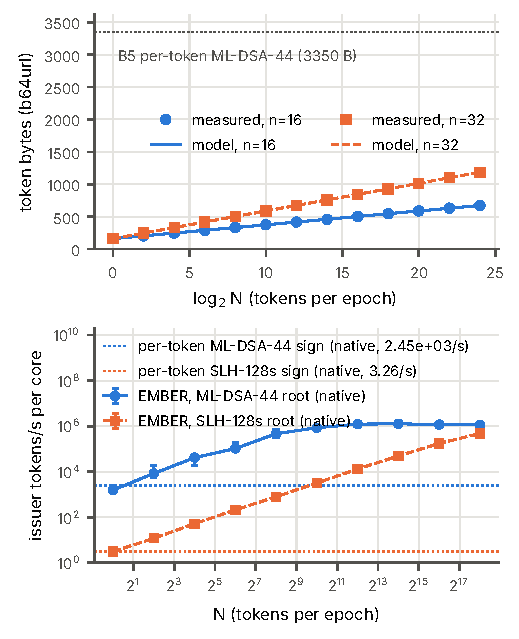
\includegraphics[width=\columnwidth]{figures/fig3_size_vs_N.pdf}
\caption{Top: EMBER token size vs.\ $\log_2 N$ (markers measured, lines Eq.~\eqref{eq:size}). Bottom: native issuer throughput per core (OpenSSL~3.5.4, run~2), with per-token signing rates as horizontal lines.}
\label{fig:sizeN}
\end{figure}

\subsection{Edge Verification Cost}
\label{sec:res-cpu}

\begin{figure*}[t]
\centering
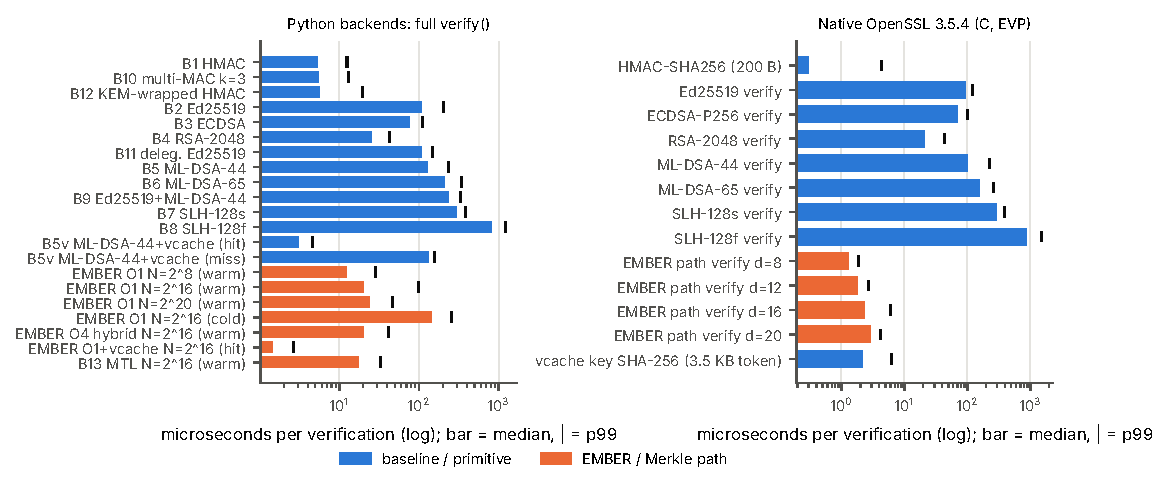
\includegraphics[width=\textwidth]{figures/fig4_verify_cost.pdf}
\caption{Per-verification cost (bar: median; tick: p99). Left: Python reference, full \texttt{verify()} (secondary source). Right: native OpenSSL~3.5.4 primitives and EMBER path verification (primary source, run~2).}
\label{fig:verify}
\end{figure*}

Fig.~\ref{fig:verify} and Table~\ref{tab:primitives} give per-verification costs. Natively, ML-DSA-44 verification takes 100.9\us{} [100.2, 120.4], close to Ed25519 (94.6\us). A warm EMBER path at $d=16$ takes 2.34\us{} [2.33, 2.46]. That is 43$\times$ cheaper than ML-DSA-44 verification, but 7.9$\times$ the 0.30\us{} of HMAC-SHA256 over the 200-B claims. Our hypothesis of at most 5$\times$ HMAC holds only for $d\le8$ (1.28\us, 4.3$\times$). Path cost grows by about 0.13\us{} per level, from 0.75\us{} at $d=4$ to 3.41\us{} at $d=24$. The Go implementation gives a smaller ratio: a full EMBER token verification (parse plus path, $N=2^{14}$) takes 3.074\us, which is 3.6$\times$ Go HMAC verification (0.853\us) and 10.7$\times$ cheaper than circl ML-DSA-44 verification (32.76\us). circl's ML-DSA-44 verification is 3.6--4.0$\times$ faster than OpenSSL's, outside the 3$\times$ cross-implementation bound we set in advance. We attribute this to circl's optimized arithmetic and report it rather than hide it.

\begin{table}[t]
\centering
\caption{Native primitive costs (OpenSSL~3.5.4, run~2; median [95\% CI], \textmu s; sizes in bytes).}
\label{tab:primitives}
\footnotesize
\setlength{\tabcolsep}{1.6pt}
\begin{tabular}{@{}lrrll@{}}
\toprule
Scheme & pk & sig & sign & verify \\
\midrule
HMAC-SHA256 & -- & 32 & 0.30 [0.30, 0.30] & 0.30 [0.30, 0.30] \\
Ed25519 & 32 & 64 & 30.1 [30.1, 30.4] & 94.6 [93.8, 96.2] \\
ECDSA P-256 & 65 & 71 & 23.0 [22.9, 31.1] & 69.6 [69.5, 70.0] \\
RSA-2048 & 270 & 256 & 314.1 [309.4, 340.5] & 20.7 [18.8, 24.2] \\
ML-DSA-44 & 1312 & 2420 & 408.8 [386.9, 452.4] & 100.9 [100.2, 120.4] \\
ML-DSA-65 & 1952 & 3309 & 676.5 [673.5, 682.7] & 154.8 [154.6, 165.8] \\
ML-DSA-87 & 2592 & 4627 & 808.7 [796.3, 871.5] & 244.8 [243.5, 250.0] \\
SLH-DSA-128s & 32 & 7856 & \num{306464} & 288.1 [282.4, 320.0] \\
SLH-DSA-128f & 32 & \num{17088} & \num{14436} & 873.2 [862.3, 883.6] \\
EMBER path $d{=}16$ & -- & 286 & -- & 2.34 [2.33, 2.46] \\
\bottomrule
\end{tabular}
\end{table}

\begin{figure}[t]
\centering
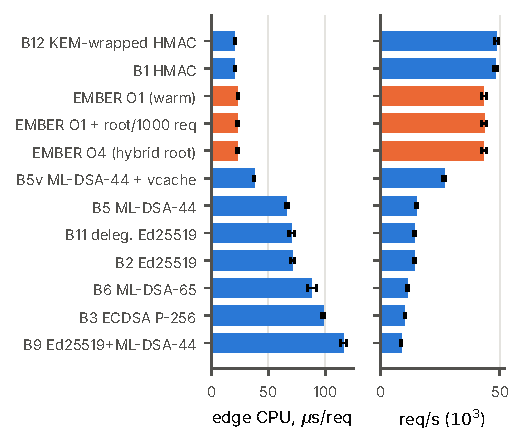
\includegraphics[width=\columnwidth]{figures/fig11_proto_capacity.pdf}
\caption{Edge capacity of the Go prototype (P1, quiet rerun, one edge core, edge utilization $\ge0.99$ in all runs; mean and 95\% $t$-CI over 5 runs). Left: edge CPU per HTTP request (primary metric). Right: requests/s.}
\label{fig:capacity}
\end{figure}

\textbf{Whole-request edge cost (P1).} Fig.~\ref{fig:capacity} shows the cost of a complete HTTP request, including Go's request parsing and response, on a single saturated edge core. Edge utilization was at least 0.99 in every one of the 60 runs. A request carrying an HMAC token (B1) costs 20.54\us{} [20.25, 20.82] of edge CPU. A warm EMBER request (O1) costs 22.91\us{} [22.49, 23.33], 1.12$\times$ HMAC, and one core serves \num{43355} req/s against \num{48340} for HMAC (0.897$\times$). Per-token ML-DSA-44 (B5) costs 66.24\us{} [65.01, 67.46], 2.89$\times$ EMBER, at \num{15040} req/s. Adding a verification cache (B5v) lowers this to 37.38\us{} (\num{26620} req/s), still 1.63$\times$ EMBER, because every request must parse and hash a 3.3~KB token. Re-verifying the root every 1000 requests (O1a, 22.92\us) or using a hybrid root (O4, 22.93\us{} [22.39, 23.47]) is indistinguishable from O1. Per-request crypto and token size, not post-quantum verification as such, determine edge cost: in Go, per-token ML-DSA-44 (66.24\us) is cheaper than Ed25519 (71.04\us), B11 (70.36\us) and ECDSA P-256 (98.04\us).

\subsection{Issuer Throughput}
Per-token ML-DSA-44 signing limits a native issuer core to $1/408.8\,\mu\text{s}\approx\num{2446}$ tokens/s. EMBER with an ML-DSA-44 root issues \num{469254} tokens/s per core [\num{319698}, \num{729692}] at $N=2^8$ and \num{1275990} [\num{1161768}, \num{1282009}] at $N=2^{14}$, 192$\times$ and 522$\times$ more (Fig.~\ref{fig:sizeN}, bottom). At large $N$ the cost is dominated by leaf hashing and base64url encoding. SLH-DSA-128s, which manages only $1/306.5\,\text{ms}\approx3.26$ tokens/s when signing per token, becomes a usable root signer: \num{49063} tokens/s at $N=2^{14}$. Its 306~ms signature, however, lies on the issuance path. In simulation it raises $D$ from 0.575~s to 0.927~s in pull mode at $\Delta=1$~s. B11 is not comparable to EMBER on issuance, contrary to our hypothesis: native Ed25519 signing (30.1\us) limits it to about \num{33000} tokens/s, so EMBER issues at least 14$\times$ faster. B12 tokens are as cheap as HMAC to issue, but every epoch requires $E$ key wraps, which take 37.6~ms at $E=500$ in our Python implementation. The Go prototype confirms the trend independently: its issuer reaches about \num{432000} tokens/s at $N=1024$, 53$\times$ its per-token ML-DSA-44 signing.

\subsection{Latency Under Load (P2)}
Over the emulated 21~ms link at 50\% of each scheme's capacity, no scheme's added median latency relative to HMAC is distinguishable from zero, except B2 ($-1.25$~ms) and B3 ($-1.39$~ms), which run at much lower absolute rates. At 80\% load, O1's median is $-3.24$~ms [$-6.82$, 0.34] relative to HMAC, while per-token ML-DSA-44 (B5) adds 11.47~ms [5.09, 17.85]. B5v's median of 80.05~ms has a CI that spans zero because individual runs collapsed. B5 and B5v are the only schemes that push 3.3~KB URLs at 9.5k and 16.4k req/s, about 260 and 450~Mbit/s of request bytes through a userspace link emulator that sustained about 624~Mbit/s in a bulk test. We therefore attribute this tail to the link emulator, not to edge CPU, but we have not verified this. All runs completed with zero errors. Load levels were set from the earlier P1 capacities.

\subsection{Dissemination and End-to-End Latency}
\label{sec:res-dissem}

\begin{figure}[t]
\centering
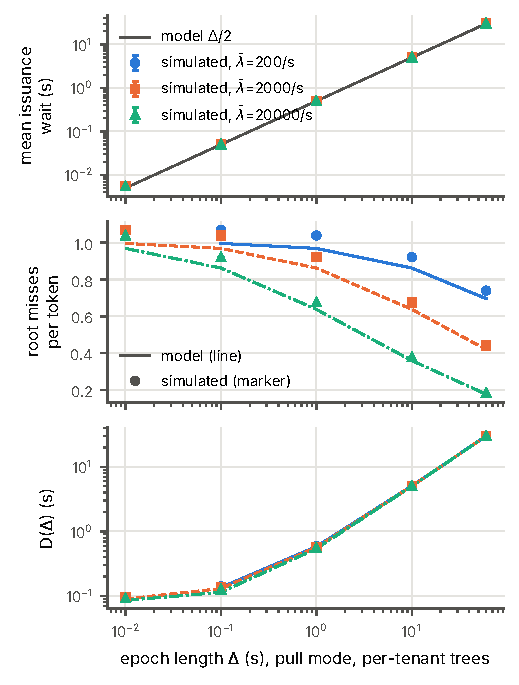
\includegraphics[width=\columnwidth]{figures/fig5_delta_tradeoff.pdf}
\caption{Pull mode, per-tenant trees (simulated, 5 seeds; model lines from Eqs.~\eqref{eq:miss}--\eqref{eq:D}). Root misses barely fall with $\Delta$ until $\lambda\Delta$ approaches $E$, so $D(\Delta)$ is minimized at the smallest $\Delta$.}
\label{fig:delta}
\end{figure}

Fig.~\ref{fig:delta} shows the trade-off that Eq.~\eqref{eq:D} predicts. Issuance wait follows $\Delta/2$. Root misses per token fall only slowly, because with $E=500$ edges and \num{1000} Zipf-distributed tenants, $\lambda_\tau\Delta\ll E$ for almost every tenant. Without re-routes the simulated misses equal Eq.~\eqref{eq:miss} to 3--4 digits. With the default mobility assumption (about 7\% of sessions switch edge once), the model under-predicts: at $\bar\lambda=2000$ and $\Delta=1$~s it gives 0.862 misses per token against 0.921 simulated.

\begin{table}[t]
\centering
\caption{Operating points (simulated; $\bar\lambda=2000$/s, $E=500$, 5 seeds, CI half-widths $<1\%$ of the mean).}
\label{tab:ops}
\footnotesize
\setlength{\tabcolsep}{3pt}
\begin{tabular}{@{}lrrrrr@{}}
\toprule
Mode & $\Delta$ (s) & misses/token & $D$ (ms) & req.\ waiting & root/served B \\
\midrule
pull & 0.01 & 1.069 & 96.2 & 0.71\% & $2.4\cdot10^{-5}$ \\
pull & 1 & 0.921 & 575.4 & -- & -- \\
pull\_staple & 0.01 & 0.073 & 11.7 & 0.049\% & $1.6\cdot10^{-6}$ \\
pull\_staple & 1 & 0.058 & -- & -- & -- \\
push & 0.01 & 0.622 & 19.8 & -- & $5.0\cdot10^{-3}$ \\
push\_rollup & 0.01 & 0.997 & -- & 0.67\% & $5.3\cdot10^{-5}$ \\
\bottomrule
\end{tabular}
\end{table}

\begin{figure*}[t]
\centering
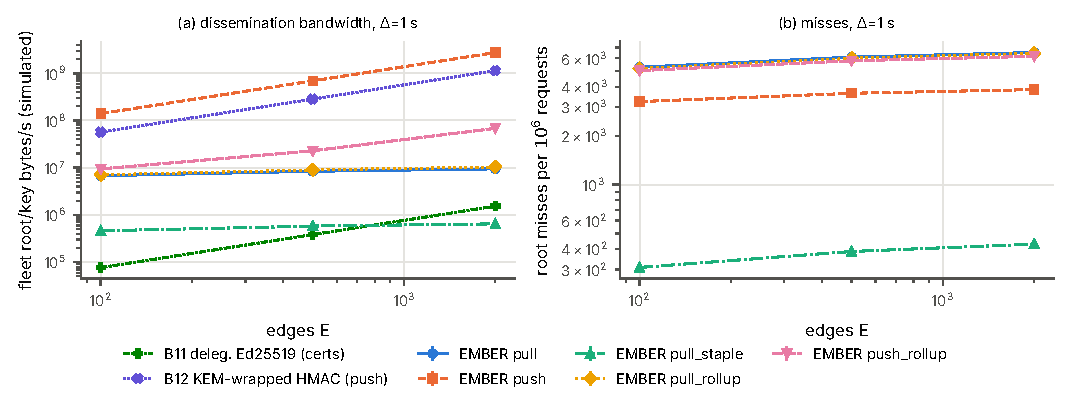
\includegraphics[width=\textwidth]{figures/fig7_dissemination.pdf}
\caption{Dissemination vs.\ fleet size ($\Delta=1$~s, $\bar\lambda=2000$/s; simulated). (a) Fleet root, key or certificate bytes/s. (b) Root misses per $10^6$ requests.}
\label{fig:dissem}
\end{figure*}

Table~\ref{tab:ops} and Fig.~\ref{fig:dissem} compare the modes. \textbf{Stapling is the decisive mode.} It reduces misses per token from 1.069 to 0.073 at $\Delta=0.01$~s, and the remaining misses come only from mid-session re-routes: 0 when no re-routes occur, 0.56 when the re-route probability is 0.005. It also cuts mean added delay $D$ from 96.2~ms to 11.7~ms and the share of requests that wait for a root from 0.71\% to 0.049\%. At $E=500$ it gives 387 misses per $10^6$ requests, against \num{6098} for pull. Root traffic is $1.6\cdot10^{-6}$ of served bytes, and fleet root bandwidth is 0.46--0.65~MB/s for $E=100$--2000. \textbf{Push} at $\Delta=0.01$~s needs 2.27~GB/s of root traffic. Even at $\Delta=1$~s it needs 140~MB/s to 2.75~GB/s for $E=100$--2000, and it still misses 0.622 per token at $\Delta=0.01$~s, because the 150~ms push delay exceeds the 120~ms between token receipt and first request. \textbf{Roll-up} did not deliver the 5$\times$ miss reduction we hypothesized. It removes only 1.4--2.2\% of misses (\num{6098}$\to$\num{6011} per $10^6$ requests at $\Delta=1$~s; 1.069$\to$1.045 misses per token at $\Delta=0.01$~s), because first requests arrive about 120~ms after issuance, before any period closes. Its value lies instead in bounding edge root state and in carrying revocation deltas (mean revocation propagation 150~s in pull modes). For comparison, B12's key-wrap push needs 57~MB/s to 1.13~GB/s and B11's certificate pulls 0.08--1.5~MB/s.

\begin{figure}[t]
\centering
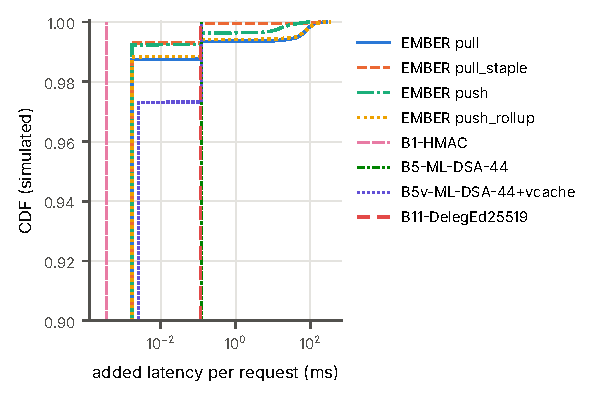
\includegraphics[width=\columnwidth]{figures/fig8_e2e_cdf.pdf}
\caption{Added latency per request (miss wait plus native verification CPU; simulated, $5\times\num{20000}$ samples per curve). Upper tail shown.}
\label{fig:e2e}
\end{figure}

Fig.~\ref{fig:e2e} shows the per-request added latency. With stapling, p99 is 0.0017~ms, 0.05\% of requests exceed 1~ms and p99.9 is 0.12~ms. Plain pull has p99 0.123~ms and p99.9 112~ms, where root-miss round trips dominate. Per-token ML-DSA-44 adds 0.122~ms to \emph{every} request, and B5v has p99 0.125~ms. Simulated edge CPU, including amortized root verification, is 1.2--1.7\us{} per request for EMBER in pull mode.

\emph{Hybrid root.} The hybrid root leaves warm per-request cost unchanged (20.27 vs.\ 19.98\us{} in Python, +1.5\%). In the Go prototype O4 and O1 differ by 0.09\% per request, with overlapping CIs (Section~\ref{sec:res-cpu}). With per-tenant trees, however, each (edge, epoch) root serves about one session, so the additional Ed25519 root verification raises \emph{simulated} mean edge CPU per request by 41.6\% (2.37 vs.\ 1.67\us). The absolute cost remains at the microsecond level, but our hypothesis of a $<1\%$ change is refuted.

\subsection{Epoch Control}
\label{sec:res-controller}

\begin{table}[t]
\centering
\caption{24-h diurnal workload, pull mode (simulated). $D$ in ms [95\% $t$-CI]. Paired: adaptive minus policy (common random numbers).}
\label{tab:controller}
\footnotesize
\setlength{\tabcolsep}{1.8pt}
\begin{tabular}{@{}lrrrr@{}}
\toprule
$\bar\lambda$ (seeds) & adaptive $D$ & best fixed $D$ & paired diff. & WC $D$ \\
\midrule
200 (10) & 96.61 & 96.61 ($\Delta$=0.01) & $-0.001$ [$-0.004$, 0.002] & 91.68 \\
2000 (10) & 96.08 & 96.08 ($\Delta$=0.01) & $+0.005$ [0.001, 0.010] & 91.68 \\
\num{20000} (5)$^\ast$ & 90.40 & 91.23 ($\Delta$=0.01) & $-0.83$ [$-0.91$, $-0.75$] & 91.45 \\
\bottomrule
\multicolumn{5}{@{}l}{\scriptsize $^\ast$1-h peak window. Best fixed $\Delta$ chosen in hindsight per rate decile.}
\end{tabular}
\end{table}

Table~\ref{tab:controller} reports hypothesis H5, which failed. The adaptive controller chose the grid floor, $\Delta=10$~ms, almost all day, and matched the best fixed $\Delta$ chosen in hindsight to within $-0.83$ to $+0.005$~ms (at most 0.9\%). This is far below the pre-registered 10~ms / 10\% threshold, so we demote the controller to a design guideline. A work-conserving close beat it by 4.93~ms and 4.41~ms at $\bar\lambda=200$ and 2000. It was 1.0~ms worse at \num{20000}, where the adaptive policy was best. Fixed $\Delta\ge3$~s violated the 2~s issuance SLO in every 5-min bin. The interior optimum predicted by Eq.~\eqref{eq:D} did not occur for any tenant at $\bar\lambda\le2000$, because misses do not fall until $\lambda_\tau\Delta\gg E$, while waiting grows linearly. With stapling, $F_{\text{miss}}$ is nearly zero, and the optimum is trivially the smallest $\Delta$ the signer sustains.

\subsection{Simulator Validation Against the Prototype}
\label{sec:res-validate}

\begin{figure*}[t]
\centering
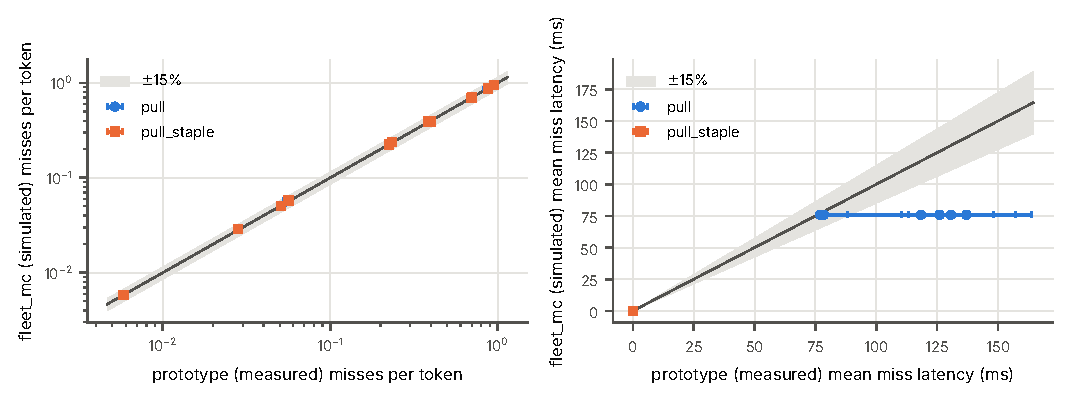
\includegraphics[width=\textwidth]{figures/fig12_proto_validation.pdf}
\caption{Simulator (fleet Monte Carlo, 50 seeds, fed measured RTTs) vs.\ prototype (P3, 5 runs, 95\% CI) on 24 configurations. Left: misses per token, 24/24 within 15\% or inside the CI. Right: mean miss latency. Pull at $\Delta\le1$~s matches; pull at $\Delta=10$~s and stapled misses do not.}
\label{fig:validate}
\end{figure*}

We ran the simulator with the prototype's P3 configuration and its measured RTT distribution, and compared it with the prototype (Fig.~\ref{fig:validate}). For \emph{misses per token} and \emph{root bytes per token}, 24 of 24 configurations pass (relative error at most 15\% or simulator inside the prototype CI). The maximum error is 4.4\% for the simulator and 14.8\% for the steady-state model, whose error at $\Delta=10$~s comes from partly filled boundary epochs in the 60~s window. For example, at $V=10$, $\Delta=1$~s and $\lambda=200$/s the prototype measures 0.05116 [0.05036, 0.05196] misses per token and the simulator predicts 0.05067. For \emph{mean miss latency}, pull at $\Delta\le1$~s passes in 8 of 8 configurations (prototype 76.9--78.5~ms, simulator 75.9~ms). The other configurations fail. Pull at $\Delta=10$~s measures 118--137~ms against 75.9~ms predicted. The four concurrent pipelines' timers are aligned, so each epoch close releases about \num{4400} tokens whose first requests reach the one-core edge within about 200~ms. First-request p50 latency is 136.8~ms at $\Delta=10$~s versus 23.6~ms at $\Delta=1$~s. The simulator has no edge-CPU or link queueing. Stapled misses measure 0.074--0.086~ms against 0.026~ms predicted, because the simulator charges only signature verification, not decoding the 3.3~KB header. That absolute gap is about 0.05~ms. We therefore scope the simulator's latency claims to non-bursty edges. Its miss and byte predictions are validated.

\subsection{Denial of Service}
\label{sec:res-dos}
We flooded one simulated edge with \num{10000} fake tokens/s. When the fake epochs are spread over all tenants, coalescing and negative caching do \emph{not} help, because keys rarely repeat: 9270--9636 root fetches/s, 4630 signature verifications/s and 0.48 of one core. Restricted to the lowest-rate tenant, coalescing reduces fetches from 7680/s to 65/s. A stapled-root flood costs \num{10000} verifications/s, 1.03 cores. A per-client limit of one staple per second (100 clients) reduces this to 100/s and 0.027 of a core. Per-client limits on fetches and staples are therefore required. Coalescing and negative caching protect only against single-tenant floods.

\subsection{Trust and Cost Summary}

\begin{table*}[t]
\centering
\caption{Trust and cost comparison. Bytes: measured token, 60-character path. Verify: native OpenSSL~3.5.4 median per request (EMBER: path, $d=16$). Dissemination: simulated fleet bytes/s for $E=500$, $\bar\lambda=2000$/s, $\Delta=1$~s.}
\label{tab:trust}
\footnotesize
\setlength{\tabcolsep}{4pt}
\begin{tabular}{@{}lllp{2.6cm}rp{2.2cm}r@{}}
\toprule
Scheme & Secret at edge & One compromised edge mints for & PQ assumption & Bytes & Verify (\textmu s) & Dissem.\ (kB/s) \\
\midrule
B1 HMAC & yes (key lifetime) & all edges, all paths of the key & unconditional & 166 & 0.30 & 0 \\
B10 multi-MAC, $k{=}3$ & yes & its own domain & unconditional & 187 & 0.30 & 0 \\
B12 KEM-wrapped HMAC & yes (epoch keys) & all edges, live epochs & unconditional (ML-KEM) & 171 & 0.30 & \num{283521} \\
B2 Ed25519 & no & none & none (Shor) & 209 & 94.6 & 0 \\
B11 delegated Ed25519 & no & none & classical security within $\vmax$ & 214 & 94.6 & 383.2 \\
B5 ML-DSA-44 & no & none & unconditional & \num{3350} & 100.9 & 0 \\
B5v + verify cache & no & none & unconditional & \num{3350} & 100.9 first, 2.19 hit & 0 \\
EMBER O1 (pull) & no & none & unconditional & 503 & 2.34 (+root per epoch) & \num{8411} \\
EMBER O1 (push) & no & none & unconditional & 503 & 2.34 & \num{689374} \\
\bottomrule
\end{tabular}
\end{table*}

Table~\ref{tab:trust} summarizes the comparison. The B5v hit cost (2.19\us) is the SHA-256 cache key over a 3.5~KB token. EMBER is not the best scheme on every metric. B11 and B12 have smaller tokens, and HMAC-based schemes have cheaper verification. Among the schemes we compared, EMBER is the only one that is at once (i) post-quantum without a time-bounded classical assumption, (ii) free of minting secrets at edges and (iii) small enough for URLs and cookies. Its costs are a root-dissemination path and tokens about 3$\times$ larger than HMAC tokens.

\section{Discussion}
\label{sec:discussion}

\begin{table*}[t]
\centering
\caption{Trust and cost comparison. Bytes: encoder URL token, 60-character path. Verify: native OpenSSL~3.5.4 medians. Dissemination: simulated fleet traffic for $E=500$ ($\bar\lambda=2000$/s) or per-session staple bytes.}
\label{tab:trust}
\scriptsize
\setlength{\tabcolsep}{3pt}
\begin{tabular}{@{}llp{2.9cm}p{2.0cm}rp{3.0cm}p{2.6cm}@{}}
\toprule
Scheme & Secret at edge & One compromised edge mints for & PQ assumption & Bytes & Verify (\textmu s) & Dissemination \\
\midrule
B1 HMAC & yes (key lifetime) & all edges, all paths of the key & unconditional & 166 & 0.30 & none \\
B10 multi-MAC, $k{=}3$ & yes & its own domain & unconditional & 187 & 0.30 & none \\
B12 KEM-wrapped HMAC & yes (epoch keys) & all edges, live epochs & unconditional & 171 & 0.30 & 283.5~MB/s key push \\
B2 Ed25519 & no & none & none (Shor) & 209 & 94.6 & none \\
B11 delegated Ed25519 & no & none & no break within $L+\vmax$ & 214 & 94.6 per (key, edge) & 0.383~MB/s ($L=1$~h) \\
B5 ML-DSA-44 & no & none & unconditional & \num{3350} & 100.9 per request & none \\
B5v + verify cache & no & none & unconditional & \num{3350} & 100.9 first, 2.19 hit & none \\
\textbf{M2} stapled ML-DSA-44 & no & none & unconditional & 148 & 100.9 per (token, edge), $\le$0.21 hit & staple \num{2921}~B/session (h2) \\
EMBER pooled, staple-all & no & none & unconditional & 268 & 0.89 path ($d{=}5$) + 100.9 per (root, edge) & staple \num{2968}~B/session (h2) \\
EMBER per-tenant, pull & no & none & unconditional & 161--247 & 0.24--0.75 path ($d{=}0$--4) + root & 8.41~MB/s ($\Delta=1$~s) \\
\bottomrule
\end{tabular}
\end{table*}

\subsection{Deployment Guidance}
Table~\ref{tab:trust} summarizes the trust and cost trade-offs. Our recommendations follow from the measurements.

\textbf{1. If edges may hold a minting key, use HMAC.} HMAC (B1) is post-quantum and the cheapest option. Per-domain multi-MAC (B10) confines a multi-CDN breach to one vendor at HMAC cost.

\textbf{2. Otherwise, staple.} Detaching the signature from the token and sending it once per edge connection fixes the edge for any signature scheme. M2 matches HMAC in edge CPU (Table~\ref{tab:p1}) and is the smallest post-quantum option in URL form; in cookie form it is within 0.4\% of the smallest (Table~\ref{tab:wire}). Clients should staple on every new edge contact, not only on the first request (Fig.~\ref{fig:pmove}). Stapling also removes the root service as an availability dependency.

\textbf{3. Batch only when the issuer is the bottleneck, and then pool.} Per-token signing costs the issuer $\lambda\times408.8$\us, about 0.41 cores per $10^3$ tokens/s per key. Pooled EMBER at $\Delta=10$~ms costs at most $1/\Delta$ root signatures per second plus hashing. In our runs this stayed at or below 0.057 cores up to \num{20000} tokens/s, and at $\lambda\ge10^3$/s trees hold at least about 10 tokens. Below about $10^3$ tokens/s per issuer key, the saving is under half a core: 0.046 cores at 200/s. That does not justify 5.4~ms of extra delay, 120--184 more bytes per token and the extra path hashing at the edge, so M2 is the better choice. Above that rate, use one pooled tree per issuer key with $\Delta\approx10$~ms and staple-all. Pooling requires that the tenants of a pool trust a shared issuer key. With per-tenant keys, batching saves only 1.2$\times$, and M2 should be used. Work-conserving closing self-limits issuer CPU to one core per pool at sub-millisecond delay (0.62~ms at \num{20000}/s), which suits pools whose rate fits on one signer core.

\textbf{4. Consider B11 if its assumption holds.} Delegated Ed25519 is smaller and cheaper to disseminate. It is appropriate when breaking one Ed25519 key is believed to take longer than $L+\vmax$ (Section~\ref{sec:res-b11}). Short $\vmax$ is the effective lever.

\textbf{5. Operational settings.} Use a node size of $n=16$ for category-1 tokens and $n=32$ above that. Add a per-$\mathit{kid}$ public seed to the tweak. Set $\vmax=1$~h and a skew tolerance $\tau=5$~s. Apply per-client limits on staples and fetches, and fetch roots only for configured $\mathit{kid}$s and recent epochs. Do not deploy per-tenant push or rely on roll-up to reduce misses.

\subsection{Limitations}
\label{sec:limits}
\begin{itemize}
\item \emph{One VM.} All prototype components share one 4-vCPU KVM guest. Network namespaces and a userspace link emulator stand in for \texttt{netem}, and there is no physical NIC and no TLS. P1 runs over loopback, so it measures edge CPU per request, not network effects. Separate P1 campaigns differed by about 10\% in absolute value.
\item \emph{Two native runs.} Absolute costs differ by 15--20\% across a VM reboot. Everything except the controller study and the simulator consistency check uses the second run (Appendix~\ref{app:secondary}).
\item \emph{Simulator scope.} The simulator is validated against the prototype only for miss and byte counts, at small scale ($V\le50$), and without re-routes or a shield tier. It has no edge-CPU or link queueing, so it under-predicts pull-miss latency for timer-aligned bursts (118--137~ms measured vs.\ 75.9~ms). Workload parameters (Zipf exponents, RTTs, $K$, $p_{\text{move}}$) are assumptions, and $p_{\text{move}}$ alone determines staple-first waiting.
\item \emph{Clients.} We tested Chrome~153, curl/nghttp2 and Go, but not Firefox or Safari.
\item \emph{Security.} We give a proof sketch, not a machine-checked proof. The public-seed variant was not implemented. Bearer-token replay is unchanged from the status quo. Pooling concentrates minting in one key.
\end{itemize}

\section{Conclusion}
\label{sec:conclusion}
Post-quantum CDN tokens have two cost centers that respond to different variables. At the issuer, the variable is the token rate per key. Pooled epoch-Merkle batching (EMBER, a CDN profile of MTL-mode batch signing) cuts issuer CPU 19--144$\times$ in simulation and needs 0.38--1.08 cores where per-token signing needs 177 at the full token rates implied by Meta's CDN traces. It pays above roughly $10^3$ tokens/s per shared key; in thin pools it saves nothing. At the edge, the variable is the number of requests $K$ a token carries at one verifier. With session tokens ($K\approx150$), stapling the signature once per connection lets per-token ML-DSA-44 cost the edge as much as HMAC, with a 148-B URL token. With one token per object per hour ($K\approx2$ on the trace), the same design verifies a signature about every second request, and a pooled tree is 28$\times$ cheaper in edge crypto and 4.4$\times$ smaller on the wire. The crossover lies at $K\approx48$--154 for CPU and 9--27 for bytes. Real token granularity is the operator's choice and is not visible in public traces. Stapled designs also make edges depend on their verified-entry caches: on our prototype, a lost entry costs one extra round trip on a live connection, a restart costs a 263~ms reconnect, and M2, which needs one entry per token, is far more sensitive to cache size than a pooled tree. Whether HPACK hides large cookies depends on the client, and delegated Ed25519 keys suffice only with a short $\vmax$. Open questions are traces with session or token identifiers, measurements in a multi-PoP deployment with re-routes, a simulator with queueing, and Firefox and Safari encoder behavior.

\section*{Data Availability}
All code, raw measurements, aggregated CSV files and figure scripts are in the author's repository. \texttt{NUMBERS\_TRACE.md} maps every number in this paper to its source file and row. [Editable: insert public archive DOI or URL before submission.]

\section*{Declaration on the Use of AI Tools}
[Editable: AI-based tools were used to assist with code, experiments and drafting. The author reviewed and takes responsibility for all content. Adapt to the venue's policy.]

\section*{Acknowledgment}
[Editable.]


\appendices
\section{EMBER Issuance}
\label{app:alg}

\begin{algorithm}[h]
\caption{Issuer: epoch closing and publication}
\label{alg:issue}
\small
\begin{algorithmic}[1]
\Procedure{Issue}{$c$}
  \State $r\gets\$\{0,1\}^{128}$; append $(c,r,\mathit{future})$ to the pool's queue $Q$; \Return await $\mathit{future}$
\EndProcedure
\Procedure{CloseEpoch}{}\Comment{timer $\Delta$, or $|Q|=N_{\max}$, or signer idle (WC)}
  \State $B\gets Q$; $Q\gets[\,]$; $e\gets e+1$; $N\gets|B|$ \Comment{rotate $\mathit{kid}$ before $e$ or $i$ wraps}
  \State $L_i\gets\Th(T_{\textsc{leaf}}(e,i),\,B[i].r\,\|\,\mathrm{enc}(B[i].c))$ for $i<N$
  \State $(R,\mathit{levels})\gets\textsc{BuildTree}(e,L)$
  \State $\sigma\gets\Sig(sk,\texttt{"EMBER-root"}\|\mathit{kid}\|e\|T_{\text{start}}\|\Delta\|N\|R)$
  \State publish $SR_e$ at \texttt{/ember/}$\mathit{kid}$\texttt{/}$e$ (immutable); push if configured
  \For{$i<N$}
    \State resolve $B[i].\mathit{future}$ with $(c_i,\mathit{kid},e,i,r_i,\textsc{Path}(\mathit{levels},i))$ and $SR_e$
  \EndFor
\EndProcedure
\end{algorithmic}
\end{algorithm}

\section{Secondary Results}
\label{app:secondary}

\emph{Epoch controller (first-run costs).} We also built an adaptive controller. It estimates the token rate with an exponentially weighted moving average and, at each epoch close, chooses $\Delta$ from a 25-point logarithmic grid in $[0.01,60]$~s to minimize $D$, subject to size, signer-capacity and 2~s issuance-latency constraints. Before the experiment we fixed a demotion rule: if the controller beat the best fixed $\Delta$, chosen in hindsight, by less than 10~ms or 10\%, it would be reported as a guideline. Over a 24-h diurnal workload in pull mode with per-tenant trees, the controller chose the grid floor of 10~ms almost all day. Its paired difference to the best fixed $\Delta$ was $-0.001$~ms [$-0.004$, 0.002] at $\bar\lambda=200$/s and $+0.005$~ms [0.001, 0.010] at 2000/s (10 seeds each), and $-0.83$~ms [$-0.91$, $-0.75$] at \num{20000}/s (5 seeds, 1-h peak). The rule therefore triggered. Work-conserving closing beat the controller by 4.93 and 4.41~ms at 200 and 2000/s, and fixed $\Delta\ge3$~s violated the SLO in every 5-min bin. These runs used first-run costs. The second-run sweep moved $D$ by at most 0.1~ms (96.17$\to$96.08~ms for pull at 10~ms), so the conclusion stands. With stapling, $F_{\text{miss}}$ is nearly zero and the optimum is simply the smallest $\Delta$ the issuer can sustain.

\emph{Simulator consistency (first-run costs).} An independent event-driven simulator agrees with the Monte Carlo engine to within 0.56\% on misses per token, 0.09\% on $D$ and 0.08\% on issuance wait, over 45 metric rows ($\bar\lambda=200$/s, $E=100$, 1~h, 5 seeds). This checks the implementation for internal consistency only. It is not a validation.

\emph{Latency under load (P2).} We ran P2 open loop over the emulated 21~ms link. Its load levels were set from an earlier, contended capacity campaign. Measured against the quiet P1 capacities, the nominal 50\% and 80\% levels correspond to 0.35--0.40 and 0.57--0.64 utilization. At about 0.6 utilization, the per-run median added p50 relative to HMAC, with [min, max] over runs, was $-2.60$~ms [$-6.29$, 0.55] for O1, +12.14~ms [3.17, 16.52] for B5 and +11.75~ms [2.61, 203.82] for B5v, one of whose runs collapsed. We attribute the B5 and B5v tails to the userspace link emulator, which carried 3.3~KB URLs at roughly 260--450~Mbit/s against about 624~Mbit/s in a bulk test. We did not verify this.

\emph{Earlier capacity campaign.} A quiet P1 campaign over 12 schemes, with edge utilization $\ge0.99$ in all 60 runs, measured edge CPU per request of 20.54\us{} for B1, 22.91 for O1, 22.93 for O4 (hybrid root), 37.38 for B5v, 66.24 for B5, 71.04 for Ed25519, 98.04 for ECDSA P-256 and 115.74 for the per-token hybrid.

\emph{Sensitivity.} An SLH-DSA-128s root puts its 306~ms signature on the issuance path and raises $D$ from 0.575 to 0.881~s (pull, $\Delta=1$~s). Halving the RTTs leaves staple-first $D$ at 0.503~s. The simulator's parameter defaults and sweep ranges are listed in Section~\ref{sec:method} and in the released \texttt{sim\_params.json}.

\section{Hypothesis Outcomes}
\label{app:hyp}

\begin{table}[h]
\centering
\caption{Hypotheses fixed before the experiments (commit \texttt{3148c65}) and their outcomes.}
\label{tab:hyp}
\footnotesize
\setlength{\tabcolsep}{2.5pt}
\begin{tabular}{@{}p{3.3cm}p{1.0cm}p{3.6cm}@{}}
\toprule
Hypothesis & Outcome & Evidence \\
\midrule
H1 EMBER token $<$512~B to $N{=}2^{20}$; $\le0.25\times$ B5c bytes/session & partly & 503~B at $2^{16}$, 588~B at $2^{20}$; 0.144$\times$ (h2 URL), 0.256$\times$ (HTTP/1.1); M2 smaller still \\
H2 verify $\le5\times$ HMAC and $\ge10\times$ cheaper than ML-DSA & partly & native 7.9$\times$ / 43$\times$; Go 3.6$\times$ / 10.7$\times$; whole request 1.15$\times$ HMAC \\
H3 issuer $\ge100\times$ per-token (Python), $N\ge2^8$ & cond. & holds at $N\ge2^8$, reached only with pooled trees \\
H4 root bytes $<0.1\%$; roll-up $\ge5\times$ fewer misses & partly & $\le1.04\cdot10^{-4}$ except per-tenant push ($5.0\cdot10^{-3}$); roll-up 1.4--2.3\% \\
H5 adaptive beats best fixed $\Delta$ & refuted & $\le$0.83~ms; demoted \\
H6 $<1\%$ requests wait; p99 edge CPU $<1$~ms & yes (model) & 0.049\% at default $p_{\text{move}}$, 0 with staple-all; p99 $\le$2.61\us \\
H7 hybrid root $<1\%$ edge cost & mixed & +0.09\% in P1; +41.1\% simulated \\
H8 simulator within 15\% of prototype & partly & misses and bytes 24/24 rows; latency 8/24 \\
H9 native issuer $\ge50\times$ per-token; B11/B12 comparable & partly & 192--522$\times$ at $N{=}2^8$--$2^{14}$; B11 issues faster than per-tenant EMBER \\
\bottomrule
\end{tabular}
\end{table}


\bibliographystyle{IEEEtran}
\bibliography{references}

\end{document}
